\documentclass[tikz,border=6pt]{standalone}
\usepackage{pgfplots}
\usepgfplotslibrary{groupplots}
\usetikzlibrary{calc}
\pgfplotsset{compat=1.18}
\begin{document}
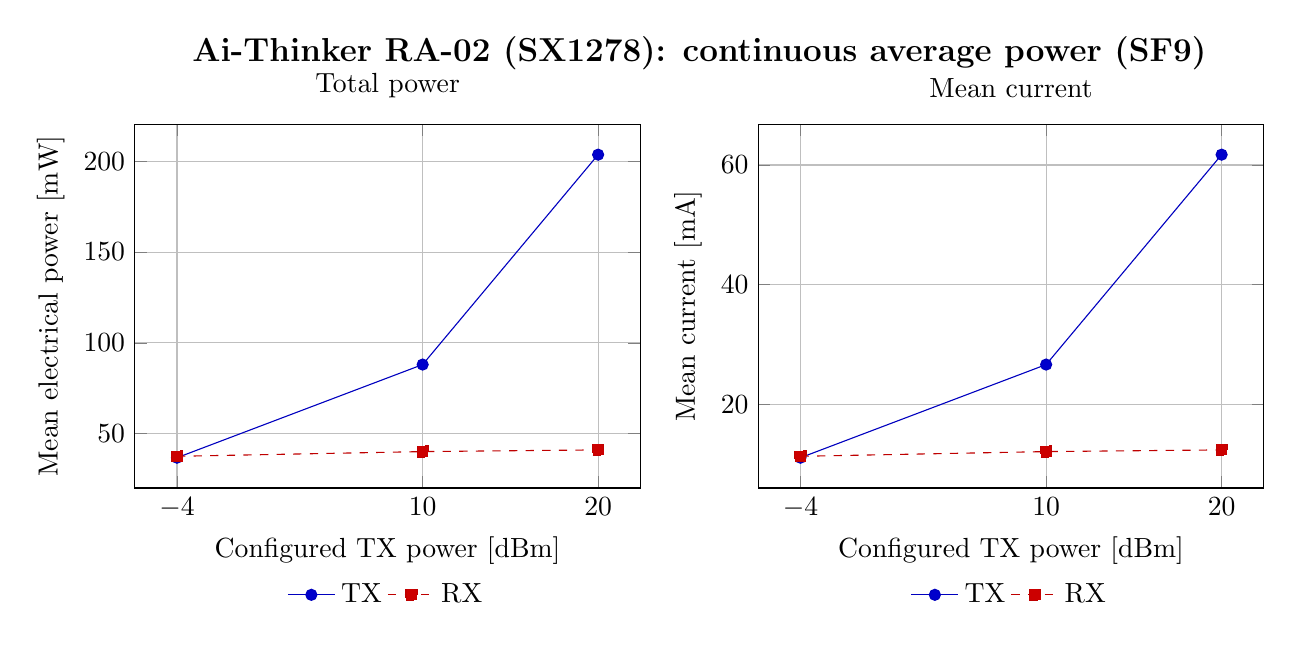
\begin{tikzpicture}
\begin{groupplot}[group style={group size=2 by 1,horizontal sep=1.5cm},width=8cm,height=6.2cm,xtick={-4,10,20},xlabel={Configured TX power [dBm]},grid=both,legend style={draw=none,at={(0.5,-0.23)},anchor=north,legend columns=2}]
\nextgroupplot[title={Total power},ylabel={Mean electrical power [mW]}]
\addplot+[blue!75!black,mark=*] coordinates {(-4,36.6514115) (10,87.9966633) (20,203.689906)};\addlegendentry{TX}
\addplot+[red!75!black,dashed,mark=square*] coordinates {(-4,37.4278852) (10,40.0308623) (20,40.9582998)};\addlegendentry{RX}
\nextgroupplot[title={Mean current},ylabel={Mean current [mA]}]
\addplot+[blue!75!black,mark=*] coordinates {(-4,11.1064883) (10,26.6656555) (20,61.7242139)};\addlegendentry{TX}
\addplot+[red!75!black,dashed,mark=square*] coordinates {(-4,11.3417834) (10,12.1305643) (20,12.411606)};\addlegendentry{RX}
\end{groupplot}
\node[font=\bfseries\large] at ($(group c1r1.north)!0.5!(group c2r1.north)+(0,0.9cm)$) {Ai-Thinker RA-02 (SX1278): continuous average power (SF9)};
\end{tikzpicture}
\end{document}
